\secnumbersection{VALIDACIÓN DE LA SOLUCIÓN}
En esta sección se presentarán los resultados obtenidos, comparando soluciones de otros métodos con las obtenidas de nuestro programa, además de hacer un análisis de recursos computacionales utilizados. Todos los cálculos de métodos variacionales cuánticos, fueron realizados utilizando el simulador \textit{default.qubit} y en condiciones sin ruido.


\subsection{Análisis de la relación hamiltoniano-\textit{ansatz}}
El objetivo de esta sección es el poder identificar regiones donde los \textit{ansazts} elegidos puedan capturar los estados de los hamiltonianos mientras variamos el valor de sus parámetros, ya que, es sabido que ciertas combinaciones de valores en los hamiltonianos pueden generar correlación mayor o menores, y es necesario saber si los \textit{ansatz} pueden o no capturarlas.

\subsubsection{Metodología}
Dado un hamiltoniano, elegimos uno de sus parámetros para analizar (en caso de tener más, los fijamos con valor arbitrario que no afecte el rendimiento). Luego se elige un conjunto de \textit{ansazt} que sean acordes al tipo de hamiltoniano. La idea es utilizar el VQE como una forma de poder analizar la relación hamiltoniano-\textit{ansatz}, ya que, si no es capaz de capturar el estado de mínima energía, es improbable que se pueda usar para métodos más avanzados (como el VQD)

Luego, para el optimizador, se utiliza un método de gradiente genérico con un \textit{learning rate} dé $0.3$. Los otros parámetros del optimizador van a ser informados en cada sección correspondiente. 

Entonces, se elige una cantidad $n$ de puntos del parámetro del hamiltoniano, para cada uno de estos se calcula el VQE $10$ veces para poder construir el promedio $\hat{x}$ y la desviación estándar $\sigma$ del valor de la energía en ese punto. Con estas dos cantidades podemos construir 3 casos en relación con el valor exacto del hamiltoniano con ese parámetro:
\begin{enumerate}
    \item Regiones de tipo 1: El valor exacto está dentro del intervalo $[\hat{x}-\sigma; \hat{x}+\sigma]$ y $|\sigma| \leq 10^{-6}$
    \item Regiones de tipo 2: El valor exacto está dentro del intervalo $[\hat{x}-\sigma; \hat{x}+\sigma]$ y $|\sigma| > 10^{-6}$
    \item Regiones de tipo 3: El valor exacto no pertenece al intervalo.
\end{enumerate}

Las regiones de tipo 1 corresponden a una situación idónea, donde las configuraciones iniciales permiten capturar de buena manera el estado de mínima energía. Las de tipo 2, muestra que, si bien es posible capturar el estado de mínima energía, uno de los hiperparámetros no es el adecuado para la tarea y este hace que se tenga una alta desviación estándar. Finalmente, las de tipo 3 se requiere un análisis un poco más detallado del porqué pareciera que el \textit{ansatz} no captura el estado. Para ello, se elige, sin pérdida de generalidad, un representante de la zona y se procede a hacer un análisis de algunos hiperparámetros para ver la razón del porqué genera esa diferencia. 


Los resultados exactos mostrados en la sección resultados, son calculados utilizando la rutina \textit{numpy.linalg.eigh} de la librería numpy para moléculas y modelos de espines, y la rutina  \textit{tenpy.algorithms.exact\_diag.ExactDiag} de la librería tenpy para los modelos de \textit{tight-binding} y Fermi-Hubbard.


\subsubsection{Definición de los sistemas}
\underline{Hamiltoniano de moléculas}: 
Para este hamiltoniano, se controlará el parámetro de distancia entre moléculas, se tendrá en consideración dos moléculas, un Hidruro de litio y un catión trihidrógeno. 


\begin{figure}[H]
\centering
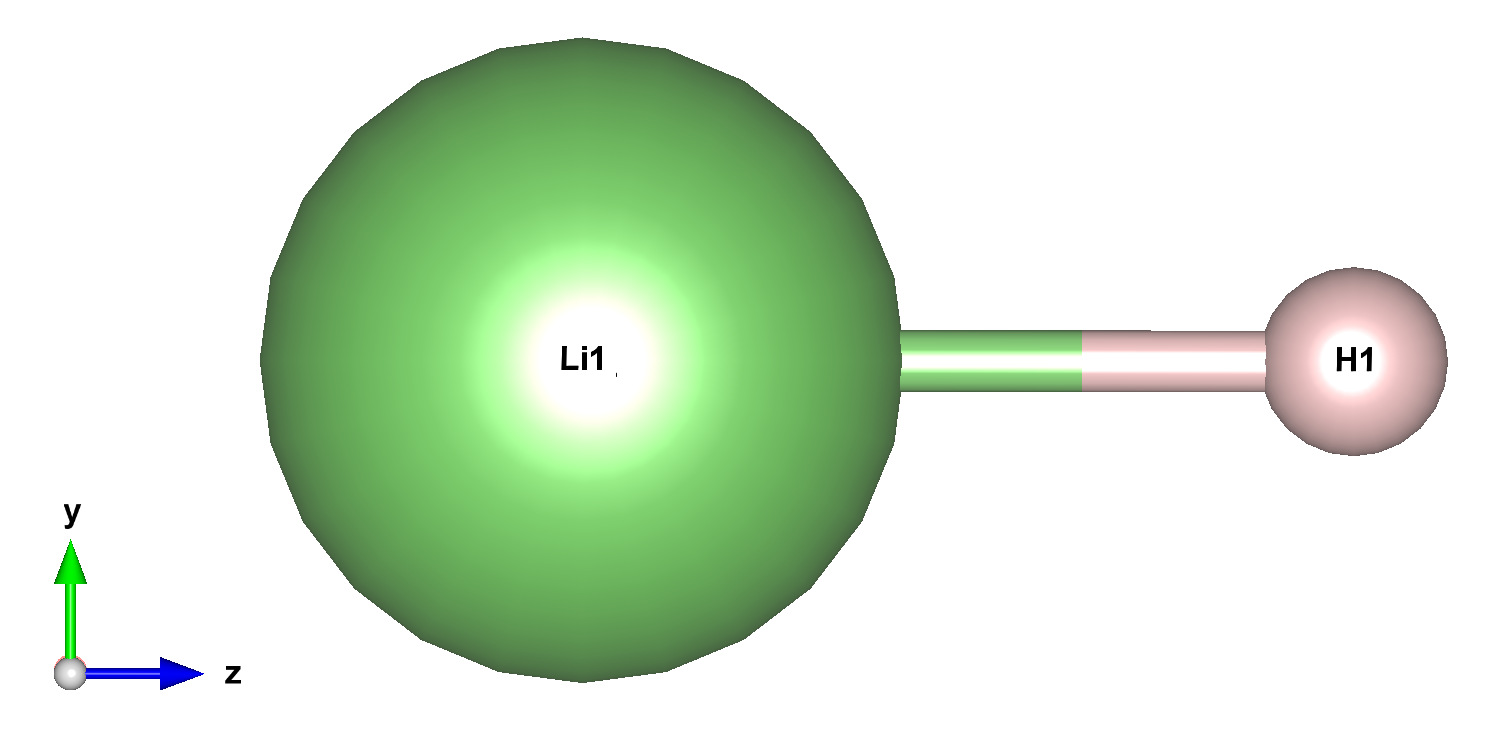
\includegraphics[width=0.5\textwidth]{figures/S4/moleculas/lih.png}
\caption{\label{fig:li} Hidruro de litio con una distancia de enlace por el eje Z. Fuente: Elaboración propia} 
\end{figure}

Para el hidruro de litio, ver figura \ref{fig:li}, se modela con los dos elementos desplazándose en el eje Z, se consideran 12 puntos del intervalo $[2;7]$, para el hamiltoniano se considera un espacio activo reducido, esto hace que el hamiltoniano se modele con 10 \textit{qubits} y 2 electrones. Por lo tanto, para el estado inicial, se considera un estado Hartree-fock de dos electrones ($\ket{1_11_20_3...0_{10}}$), el cual es utilizado en los \textit{ansatz} UCCSD y k-UpCCGSD (ambos con una repetición).

\begin{figure}[H]
\centering
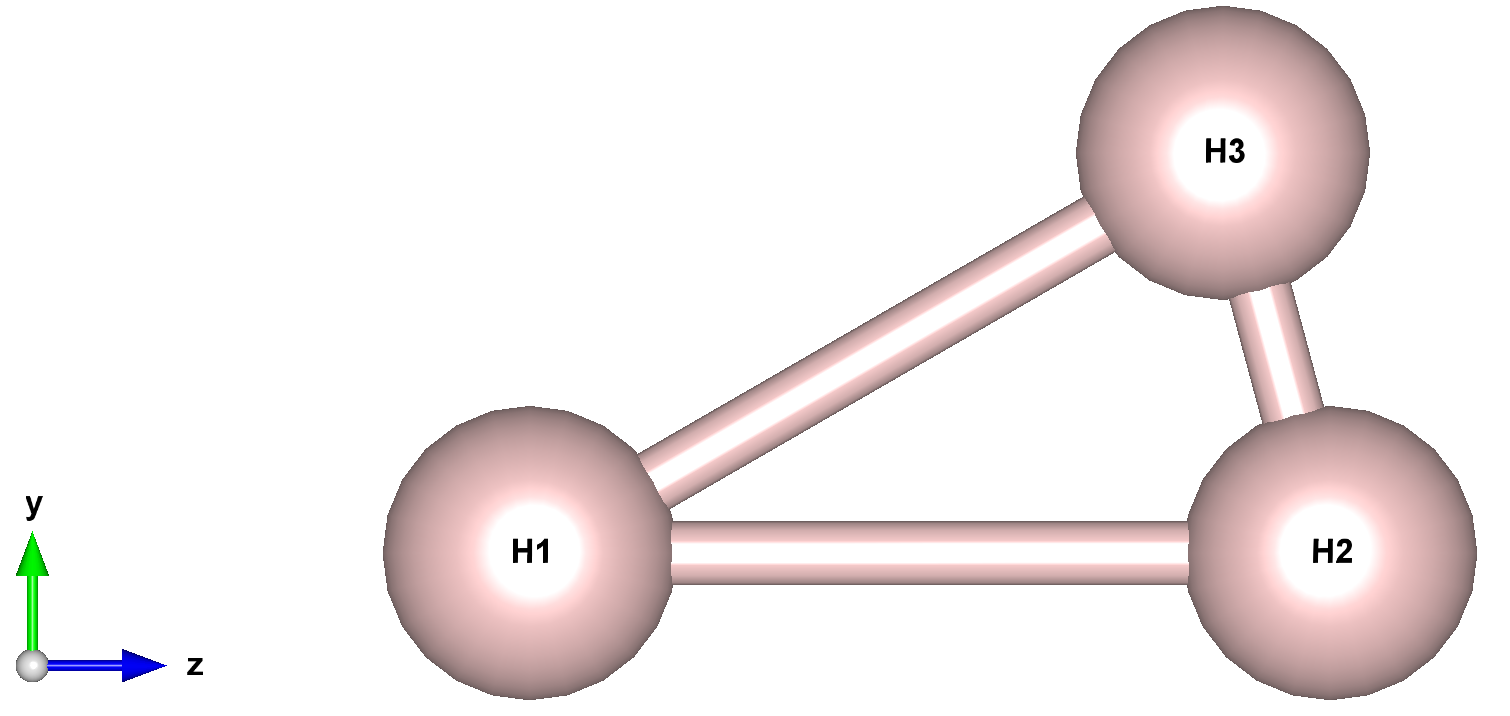
\includegraphics[width=0.5\textwidth]{figures/S4/moleculas/3h.png}
\caption{\label{fig:3h} Catión trihidrógeno modelado con un triángulo isósceles en el plano YZ. Fuente: Elaboración propia} 
\end{figure}

Para el catión trihidrógeno, ver figura \ref{fig:3h}, se modela como un triángulo isósceles en el plano YZ, se consideran 14 puntos del intervalo $[1.5; 8]$, para el hamiltoniano se considera un espacio activo completo con carga 1, ya que al ser un catión tiene un electrón menos, esto hace que el hamiltoniano se modele con 6 \textit{qubits} y 2 electrones. Para el estado inicial se considera un estado Hartree-fock de dos electrones ($\ket{1_11_20_3...0_{6}}$) que corresponde al número de electrones de valencia. Este estado inicial es utilizado en los \textit{ansatz} UCCSD y k-UpCCGSD (ambos con una repetición)

Para el optimizador, se consideran $60$ iteraciones máximas con una tolerancia dé $10^{-6}$.

\underline{Hamiltoniano de Fermi-Hubbard}: 
Para este hamiltoniano se consideran dos casos de interés, uno donde se controla el parámetro de \textit{hopping} $-t$ y otro donde se controla el parámetro de potencial $U$.

Para el primer caso, se consideraron 12 puntos del parámetro de \textit{hopping} $-t$ en el intervalo $[-1.5; 1.5]$ con un potencial $U=0$. Se consideraron los \textit{ansatz} UCCSD y k-UpCCGSD con una repetición, los cuales son inicializados en un estado Hartree-fock con un número de electrones igual a la cantidad de sitios (condición de \textit{half-filling}).

Para el segundo caso, el parámetro de \textit{hopping} se fija en el valor $-1$ y para el parámetro del potencial se consideran 6 puntos en el intervalo $[0;1]$. Se consideraron los \textit{ansatz} UCCSD y k-UpCCGSD con una repetición, los cuales son inicializados en un estado Hartree-fock con un número de electrones igual a la cantidad de sitios (condición de \textit{half-filling}).

Para ambos casos, se consideran sistemas de tamaños $3$ hasta $6$ y el optimizador tiene un límite de 100 iteraciones y una tolerancia dé $10^{-6}$.

\underline{Hamiltoniano de espín}: 
Para este hamiltoniano se controlará el parámetro $J$ usando un modelo XXX, el cual corresponde a un modelo donde todos los ejes tienen el mismo valor de \textit{exchange}. El parámetro $J$ puede tomar valores dentro de $[-1.5; 1.5]$ y se considerarán 13 puntos dentro del intervalo. 

Lo anterior va a hacer realizado en sistemas de $9$ a $12$ espines con condiciones abiertas y cerradas (una cadena y un anillo). Las ejecuciones van a ser llevadas a cabo considerando un estado inicial $\ket{0_10_2...0_{n-1}0_n}$, el \textit{ansatz hardware efficient} con una repetición. Para el optimizador, se consideran $100$ iteraciones máximas con una tolerancia dé $10^{-6}$.


\subsubsection{Resultados numéricos}
Considerando las condiciones antes expuestas, ahora se presentarán los resultados obtenidos para cada uno de los hamiltonianos.

\underline{Hamiltoniano de moléculas}:

\begin{figure}[H]
\centering
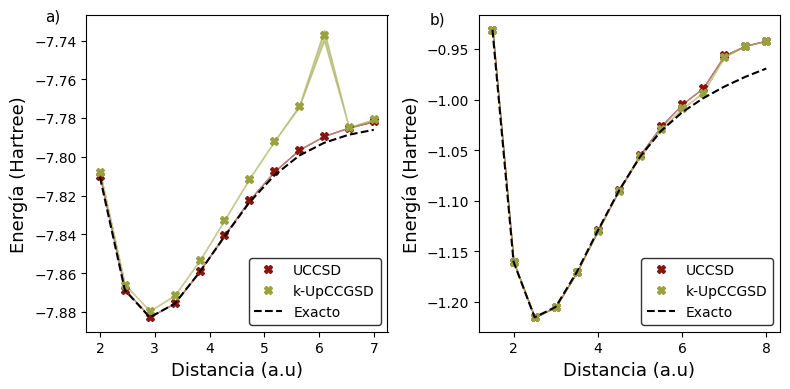
\includegraphics[width=0.9\textwidth]{figures/S4/moleculas/barridomoleculas.png}
\caption{\label{fig:5} VQE aplicado a a) $LiH$ y b) $H_3^{+}$ a distintas distancias entre moléculas. Fuente: Elaboración propia} 
\end{figure}

En la parte a) de la figura \ref{fig:5}, se puede ver como los mejores resultados se obtienen cerca del mínimo (es decir, en la distancia de equilibrio), al salir de esta región, se ve el \textit{ansatz} UCCSD presenta mejores resultados hasta donde ya el sistema se puede considerar dos moléculas aisladas. En el caso del k-UpCCGSD, se ve un aumento del error de forma considerable en zonas cercanas al mínimo, mostrando así un mal funcionamiento (alrededor de las $3.5$ (a.u)).

Pasando a la imagen b), vemos que ambos \textit{ansatz} presentan un buen rendimiento cerca del punto de equilibrio, solo cuando los hidrógenos están ya muy alejados entre sí, se ve un error perceptible. Esta mejora del k-UpCCGSD se puede explicar por la baja dimensionalidad del sistema.

Basándonos en que el UCCSD tiene un buen rendimiento en un rango amplio centrado en el punto de equilibrio, no es necesario realizar un análisis, ya que, es raro estudiar moléculas tan alejadas del mínimo. Por otro lado, si tomaremos el k-UpCCGSD para ver el porqué de la diferencia en el mínimo de la molécula $LiH$ (constituye una región del tipo 2). Dicho esto, consideraremos la distancia de equilibrio de $2.969280527$ (a.u) ($5.5822473$ (ángstrom)) para el \textit{basis set} ''sto-3g'' indicada en la CCCBD \cite{CCCBDB}. 


En la figura \ref{fig:10}, se puede el efecto de aplicar repeticiones al \textit{ansatz} (además de modificar el \textit{learning rate} a $0.2$ y aumentar el número de iteraciones a 100), en ninguno de los casos se ve una mejora sustancial de la solución, observando la gráfica del error se ve que después de la caída abrupta el error empieza a decaer muy lentamente, hasta las 100 iteraciones, no se ve ningún estancamiento que permita generar conclusiones respecto al \textit{ansatz}. Pero, como requiere tantas iteraciones, esto nos indica que no es un \textit{ansatz} adecuado para esta molécula. 

\begin{figure}[H]
\centering
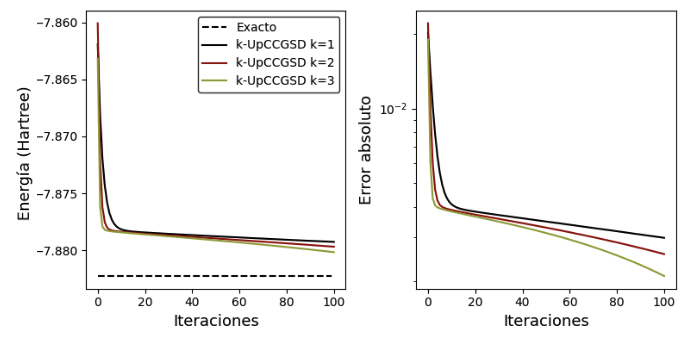
\includegraphics[width=0.9\textwidth]{figures/S4/moleculas/barridomoleculas2.png}
\caption{\label{fig:10} VQE aplicado a $LiH$ con diferentes repeticiones. Fuente: Elaboración propia}
\end{figure}


\underline{Hamiltoniano de Fermi-Hubbard}:

En la figura \ref{fig:6}, se puede observar el comportamiento del VQE sobre el modelo de \textit{tight binding}. Partiendo con el \textit{ansatz} UCCSD, se ve que este es capaz de capturar sin problemas las correlaciones independientes del tamaño y condiciones de borde, aunque para valores pequeños de $t$, se ven pequeñas diferencias respecto al valor exacto. Luego, si pasamos al \textit{ansatz} k-UpCCGSD, tenemos una situación similar, con la diferencia que para valores $|t|>1$, el \textit{ansatz} da malos resultados (ver cadena de 6 sitios), pero para valores menores a 1, presenta un rendimiento similar al UCCSD.

\begin{figure}[H]
\centering
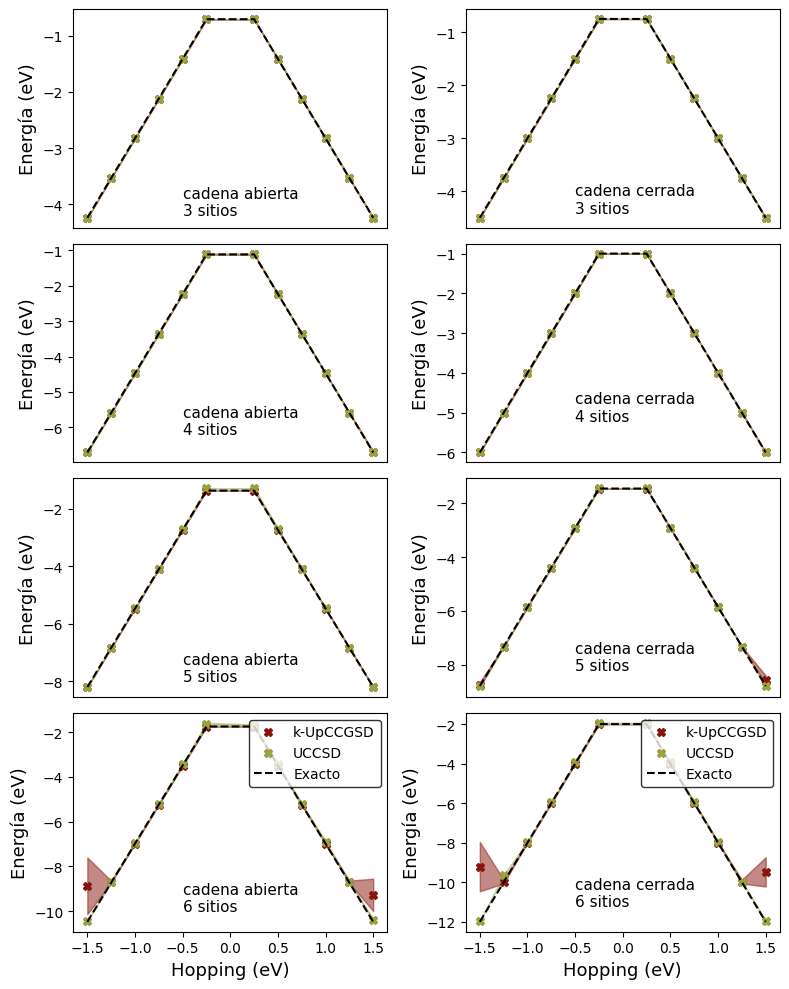
\includegraphics[width=0.8\textwidth]{figures/S4/tb/barridotb.png}
\caption{\label{fig:6} VQE aplicado a diferentes valores de $t$ con $U=0$ (\textit{tight biding}). Fuente: Elaboración propia}
\end{figure}

Para factores prácticos, nos es útil que se tenga un buen rendimiento para valores $t=1$, ya que, en la práctica, es común cocientar el hamiltoniano para que el término de \textit{hopping} sea igual a 1 (pero esto es solo posible, si él $t$ es el mismo para cada sitio, lo cual puede variar en algunas ocasiones). Es por ello por lo que, en vez de concentrarnos sobre el error en los valores grandes, nos concentraremos en el error en los valores cercanos a 0. Dicho esto, sin pérdida de generalidad, tomaremos una cadena de 5 sitios con condiciones de borde abiertas y un \textit{hopping} $t=0.15$, para este análisis solo consideraremos el \textit{ansatz} UCCSD (ya que este es el que presenta diferencias sustanciales al valor exacto). Como no es posible aplicar repeticiones a esta \textit{ansatz}, se estudiarán otros hiperparámetros.

\begin{figure}[H]
\centering
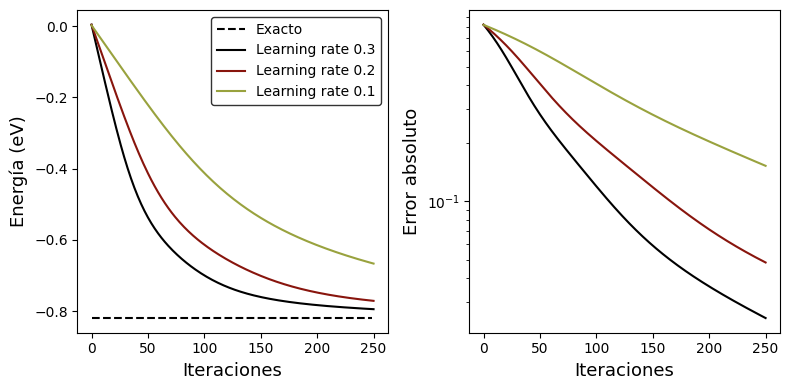
\includegraphics[width=0.9\textwidth]{figures/S4/tb/barridotb2.png}
\caption{\label{fig:11} VQE aplicado al modelo \textit{tight binding} con $t=0.15$. Fuente: Elaboración propia}
\end{figure}

En la figura \ref{fig:11} se pueden ver los efectos de modificar el \textit{learning rate} del optimizador, en ninguno de los casos se ve una mejora sustancial, lo cual nos indica que el \textit{ansatz} con una sola repetición no es capaz de capturar el estado de mínima energía cuando él $|t|<< 1$.

\begin{figure}[H]
\centering
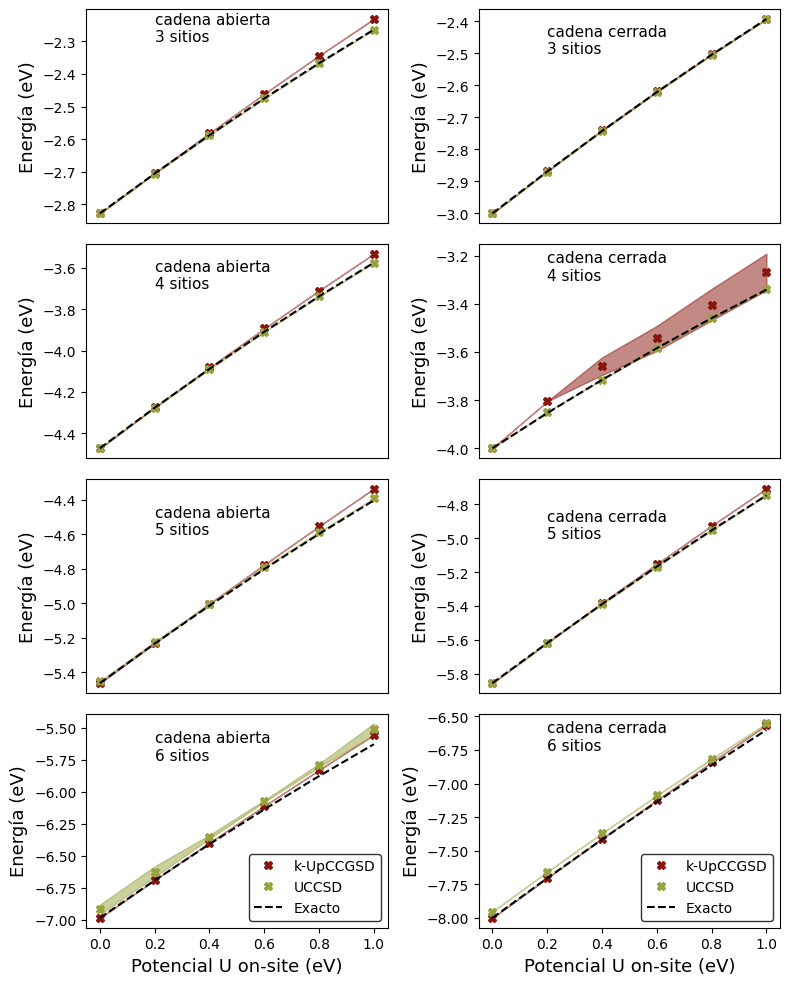
\includegraphics[width=0.9\textwidth]{figures/S4/fermi/barridofh.png}
\caption{\label{fig:7} VQE aplicado a diferentes valores de $U$ con $t=1$ (Fermi-Hubbard). Fuente: Elaboración propia}
\end{figure}

Pasando al modelo de Fermi-Hubbard, con $t=1$, encontramos un resumen de los valores obtenidos en la figura \ref{fig:7}. De esta imagen se puede observar cómo los mejores resultados se obtienen del \textit{ansatz}  k-UpCCGSD dentro de un intervalo entre 0.0 y 0.4 aproximadamente (ignorando el caso con 4 sitios y condiciones de borde cerrada), fuera de este rango, se ve como las curvas se empiezan a separar de la línea del valor exacto.

Cuando vamos aumentando el tamaño del sistema, se observa como el UCCSD va dando soluciones peores en contraste al otro \textit{ansatz} (esto, dentro y fuera del rango mencionado en el párrafo anterior), independiente de las condiciones de borde y del valor del potencial. A continuación, analizaremos el caso particular de k-UpCCGSD para 4 sitios en la cadena cerrada para el valor de $U=0.4$, y para el UCCSD consideraremos el caso de 6 sitios con condiciones de borde abierta y un valor dé $U=0.0$.

\begin{figure}[H]
\centering
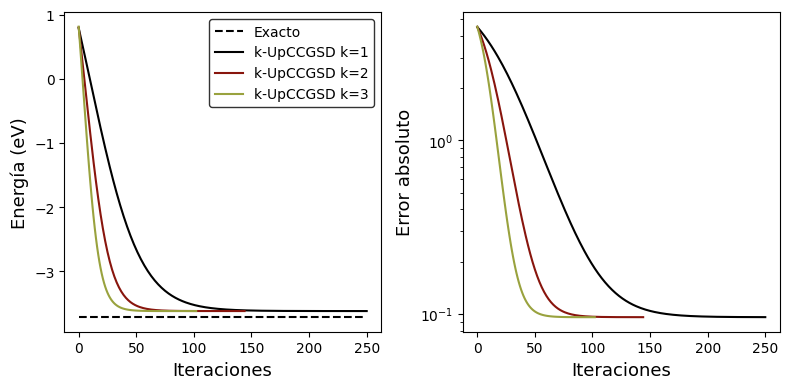
\includegraphics[width=0.9\textwidth]{figures/S4/fermi/barridofh2.png}
\caption{\label{fig:12} VQE aplicado al modelo de Fermi-Hubbard de 4 sitios con condiciones de borde cerradas con $t=1$ y $U=0.4$ y \textit{ansatz} k-UpCCGSD. Fuente: Elaboración propia}
\end{figure}

En la figura \ref{fig:12} se puede observar como a pesar de aumentar el número de repeticiones (además de aumentar el número de iteraciones a 250 y disminuir el \textit{learning rate} a $0.01$) del \textit{ansatz}, no se ve una mejora sustancial en el error, solo se aprecia una convergencia más rápida al mínimo que el \textit{ansazt} puede calcular (cantidad que varía del valor exacto). Viendo este comportamiento, es posible indicar que este \textit{ansatz} para ese caso particular, no es el adecuado, existe una incapacidad del \textit{ansatz} para capturar correctamente el estado de mínima energía.

\begin{figure}[H]
\centering
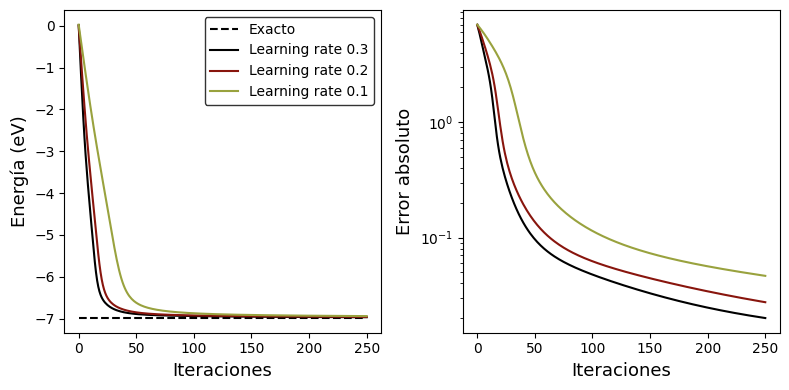
\includegraphics[width=0.9\textwidth]{figures/S4/fermi/barridofh3.png}
\caption{\label{fig:13} VQE aplicado al modelo de Fermi-Hubbard de 6 sitios con condiciones de borde abiertas con $t=1$ y $U=0.0$, y \textit{ansatz} UCCSD. Fuente: Elaboración propia}
\end{figure}

Ahora, pasando al siguiente caso, en la figura \ref{fig:13} se puede observar los efectos de la variación del \textit{learning rate} (además de aumentar el número de iteraciones a 250) sobre el cálculo del estado de mínima energía. En ninguno de los casos se observa una mejora sustancial, solo mediante el aumento del número de iteraciones se ve como el error absoluto va disminuyendo, pero esto genera problemas de viabilidad por el alto número de iteraciones requeridas para alcanzar el error buscado. Es por ello por lo que se puede indicar que este \textit{ansazt} no es el adecuado para este sistema cuando el número de sitios aumenta.

\underline{Hamiltoniano de espín}: 
En la figura \ref{fig:1}, se puede observar los resultados obtenidos para sistemas de distinto tamaño y de diferentes condiciones de borde, mientras se varía el \textit{exchange} $J$. Uno de los detalles que se observa a simple vista es para valores positivos de \textit{exchange} se observan valores que solapan el valor exacto y tienen una desviación de estándar menor que la tolerancia (región de tipo 1). Mientras que para valores negativos se observa, de manera preliminar, que el promedio no captura el valor exacto, además de tener desviaciones estándar por sobre la tolerancia (región de tipo 3). Ambas situaciones parecen ser independientes del tamaño y de las condiciones de borde.

\begin{figure}[H]
\centering
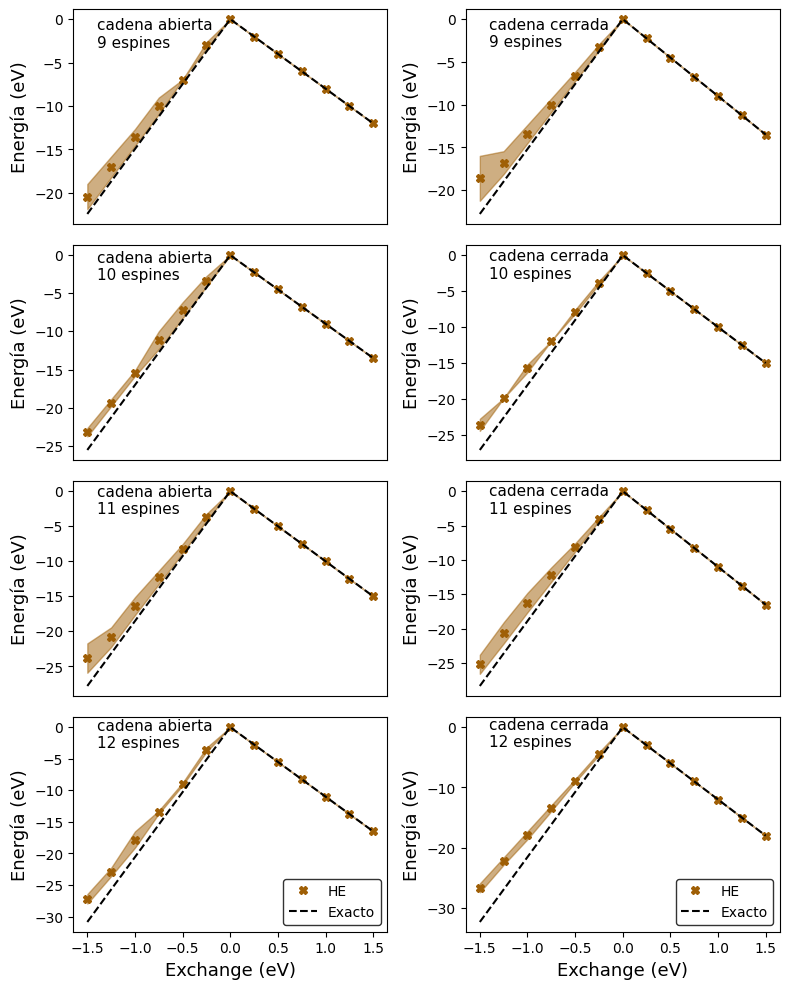
\includegraphics[width=0.9\textwidth]{figures/S4/spins/barridoespines.png}
\caption{\label{fig:1} VQE aplicado la modelo de espines a diferentes valores de $J$. Fuente: Elaboración propia}
\end{figure}

Dicho lo anterior, los valores positivos corresponden a una región de tipo 1, mientras que los valores negativos corresponden a una de tipo 3, por lo tanto, es necesario realizar un análisis más detallado para este tipo de valores.

Entonces, sin pérdida de generalidad, se toma una cadena abierta de 9 espines con un valor de \textit{exchange} $J=-1$ (eV) (modelo XXX). En la figura \ref{fig:8} se puede observar la convergencia del VQE a medida que aumentamos las repeticiones del \textit{ansatz} para alcanzar correlaciones más complejas, a pesar de esto, en la gráfica del error absoluto se ve como ninguna de estas parece alcanzar una rápida convergencia, además de mostrar síntomas de estancamiento a medida que aumentamos el número de iteraciones.

\begin{figure}[H]
\centering
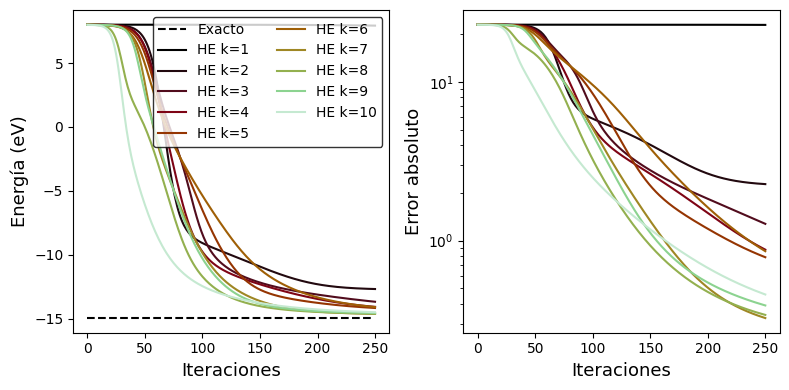
\includegraphics[width=0.9\textwidth]{figures/S4/spins/barridoespines2.png}
\caption{\label{fig:8} VQE aplicado al modelo de espines considerando 9 espines con $J=-1$ (eV) y condiciones de borde abierta. Acá se consideran 250 iteraciones y un \textit{learning rate} de $0.01$. Fuente: Elaboración propia}
\end{figure}

\begin{figure}[H]
\centering
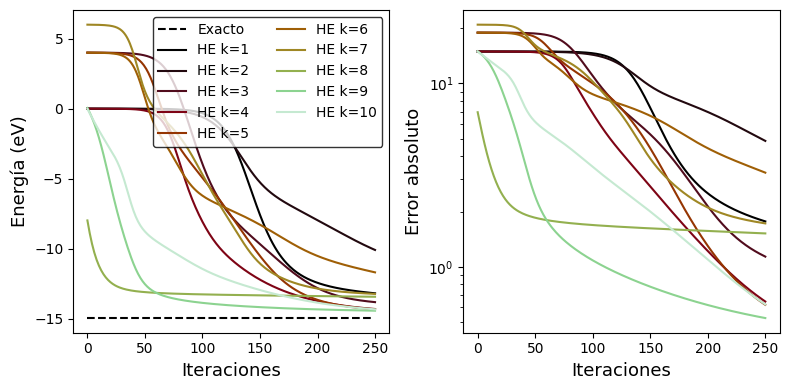
\includegraphics[width=0.9\textwidth]{figures/S4/spins/barridoespines3.png}
\caption{\label{fig:9} VQE aplicado al modelo de espines considerando 9 espines con $J=-1$ (eV) y condiciones de borde abierta. Acá se consideran 250 iteraciones, un \textit{learning rate} de $0.01$ y un estado inicial $\ket{010101010}$. Fuente: Elaboración propia}
\end{figure}

En consideración que al variar estos parámetros no hay ninguna mejora, lo otro que se tiene que probar es el punto inicial, en la figura \ref{fig:9} se puede ver los efectos del cambio inicial, pero, a pesar de ello, ninguno muestra una tendencia de la cual se puede esperar que alcance la tolerancia buscada. Por lo tanto, acá se puede concluir que el problema es la capacidad del \textit{ansatz} de capturar el estado de mínima energía, ya que, la otra opción es aumentar el número de repeticiones, lo cual puede llegar a ser muy costoso.













%%
%%
%%
%%
\subsection{Análisis de uso de memoria}
En esta sección, lo que se busca es el poder comparar de forma cuantitativa el uso de memoria que puede requerir el almacenamiento del hamiltoniano utilizando diferentes técnicas de representación. Como acá estamos comparando requerimientos de memoria, se eligen valores arbitrarios para los parámetros del hamiltoniano.

\subsubsection{Metodología}
En esta sección se busca comparan 4 representaciones posibles de un hamiltoniano, una matricial, otra en listas de cadenas de Pauli, otra en MPS/MPO y finalmente la representación que utilizan por defecto en Pennylane.

Para la matricial, se calculará de forma teórica el uso de memoria, considerando que cada elemento de esta es un número de 8 \textit{bytes} (\textit{float64}). Para la representación de MPO, utilizaremos la librería de python tenpy que implementa las redes tensoriales que son utilizadas para la construcción MPS, MPO y ejecución de DMRG. 

Para las representaciones de MPO, de Pennylane y la de listas de cadenas de Pauli, se utilizará la función \textit{asizeof} de la librería de python pympler. La idea es analizar el crecimiento de uso de memoria a medida que aumentamos el tamaño del sistema.

Por temas de notación, ''pennylane'' hace referencia a la representación de Pennylane, ''tenpy'' hace referencia a la representación MPS/MPO, ''matriz'' hace referencia al cálculo antes mencionado y ''nuestra clase'' hace referencia a la lista de cadenas de Pauli.

\subsubsection{Definición de los sistemas}

\underline{Hamiltoniano de moléculas}:
Para este hamiltoniano, se considerarán dímeros de elementos entre el hidrógeno y el nitrógeno, estos hamiltonianos son construidos utilizando todo el espacio activo, considerando el \textit{basis set} sto-3g. Todos estos dímeros son construidos considerando una distancia de $1.5$ (a.u) entre los átomos.

Para este hamiltoniano se considerarán tres representaciones, la representación matricial, la representación de Pennylane y la representación en lista de cadenas de Pauli. No se tiene en cuenta la representación MPS/MPO porque esta no tiene una implementación directa para moléculas, es por ello por lo que se decidió no utilizarla, ya que se escapa de los alcances de la memoria.

\underline{Hamiltoniano de Fermi-Hubbard}:
Para este hamiltoniano, se consideran dos casos, el primero es considerando valores $t=1$ y $U=0.0$, el segundo es con valores $t=1$ y $U=2.0$ (el primero caso corresponde al modelo \textit{tight biding} y el segundo corresponde al modelo Fermi-Hubbard). En ambos casos, se tiene una estructura de anillo, ya que esta tiene más términos que una cadena y sirve como una cota superior para sistemas de cadenas.

Para este hamiltoniano se considerarán cuatro representaciones, la representación matricial, la representación de Pennylane, la representación en MPS/MPO y la representación en lista de cadenas de Pauli.

\underline{Hamiltoniano de espín}: 
Para este hamiltoniano, se considera un modelo de espines XXX (mismo \textit{exchange} para todos los ejes) con un valor $J=1$ (eV). Al igual que para el hamiltoniano anterior, se considera una estructura de anillo.

Para este hamiltoniano se considerarán cuatro representaciones, la representación matricial, la representación de Pennylane, la representación en MPS/MPO y la representación en lista de cadenas de Pauli.


\subsubsection{Resultados de uso de memoria}
\underline{Hamiltoniano de moléculas}:

\begin{figure}[H]
\centering
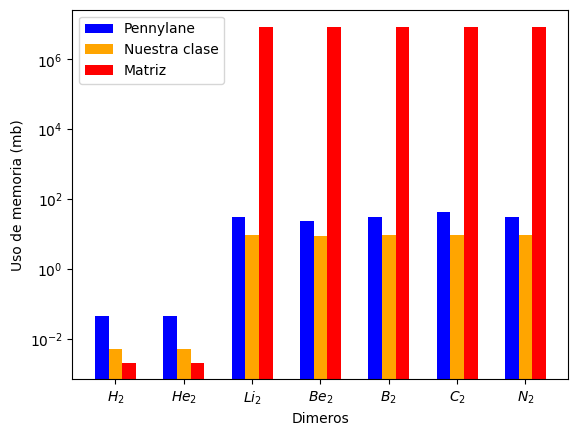
\includegraphics[width=0.7\textwidth]{figures/S4/moleculas/usomemoriamols.png}
\caption{\label{fig:20} Uso de memoria de los diferentes hamiltonianos de dímeros en (mb). Fuente: Elaboración propia}
\end{figure}

En la figura \ref{fig:20} se puede observar la diferencia de requerimientos de memoria que cada hamiltoniano necesita para almacenarse en una variable durante los flujos de cálculo. Para sistemas de baja dimensionalidad ($H_2$ y $He_2$ que requieren 4 \textit{qubits}), las matrices son menos costosa que las otras representaciones, pero cuando pasamos a sistemas más grandes, se aprecia una clara diferencia, donde nuestra representación y la de Pennylane ofrecen un uso más eficiente de recursos. Entre ambas, la diferencia no es muy sustancial, pero nuestra representación ofrece un uso de memoria menor.

En ninguno de los casos se observa una tendencia, ya que los hamiltonianos están a base de los orbitales que tienen cada elemento, por lo tanto, para establecer un flujo se tendría que seleccionar sistemas que tengan diferentes consideraciones de orbitales.



\underline{Hamiltoniano de Fermi-Hubbard/\textit{tight binding}}:

\begin{figure}[H]
\centering
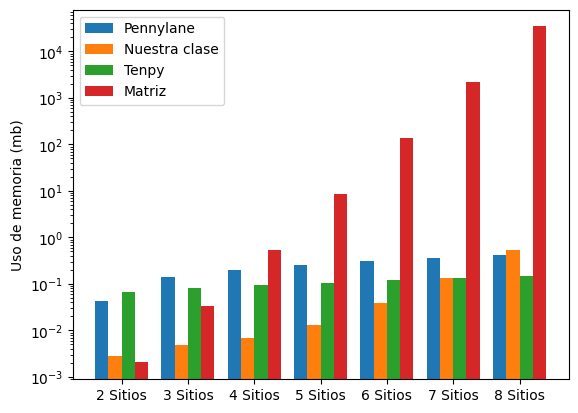
\includegraphics[width=0.7\textwidth]{figures/S4/tb/usomemoriatb.png}
\caption{\label{fig:21} Uso de memoria del hamiltoniano \textit{tight binding} a diferente número de sitios en (mb). Fuente: Elaboración propia}
\end{figure}


Para el caso del modelo de \textit{tight binding}, podemos visualizar en la figura \ref{fig:21}, los costos de memoria asociados a mantener el hamiltoniano almacenado en el flujo. En comparación a almacenar la matriz completa, las otras representaciones muestran un consumo menor. Si concentramos el análisis en las tres representaciones, vemos que tanto tenpy como Pennylane ofrecen una representación con consumos similares, en contraste con la nuestra, para menos de 8 sitios se ve una mejora, mientras que, para más de 8 sitios, nuestra representación muestra un consumo superior, pero no es una diferencia sustancial. 

La representación matricial muestra una tendencia lineal, considerando que la escala de la gráfica es logarítmica, mientras que Pennylane y tenpy muestran tendencias logarítmicas. Finalmente, nuestra representación tiene una tendencia que parece una mezcla entre lineal y exponencial, pero, para poder hablar de una forma más certera, se requiere aumentar la cantidad de sitios.

\begin{figure}[H]
\centering
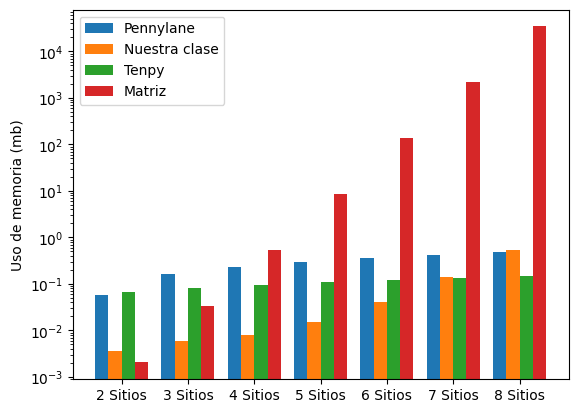
\includegraphics[width=0.7\textwidth]{figures/S4/fermi/usomemoriafh.png}
\caption{\label{fig:22} Uso de memoria del hamiltoniano Fermi-Hubbard a diferente número de sitios en (mb). Fuente: Elaboración propia}
\end{figure}


Ahora, pasando al modelo de Fermi-Hubbard, el resumen de costos se puede observar en la figura \ref{fig:22}. Como el modelo de Fermi-Hubbard es esencia, el modelo de \textit{tight biding} con unos cuantos términos extras, la tendencia es similar. Las representaciones de Pennylane y tenpy ofrecen rendimientos similares, que, en contraste con la nuestra, están muy cercanas.


\underline{Hamiltoniano de espín}:
Para el caso del modelo de espines XXX, el resumen de costos se puede observar en la figura \ref{fig:23}. Al igual que en los sistemas anteriores, la representación matricial es la que más recursos utiliza. Dejando está de lado, las representaciones de Pennylane y tenpy ofrecen un consumo considerablemente inferior a la matricial. Finalmente, nuestra representación ofrece un consumo inferior a las anteriores mencionadas, pero a medida que aumenta el número de espines esta es muy cercana al consumo de Pennylane y tenpy. Al igual que con los modelos anteriores, se aprecia como nuestra representación muestra tendencias entre lineales y exponenciales.


\begin{figure}[H]
\centering
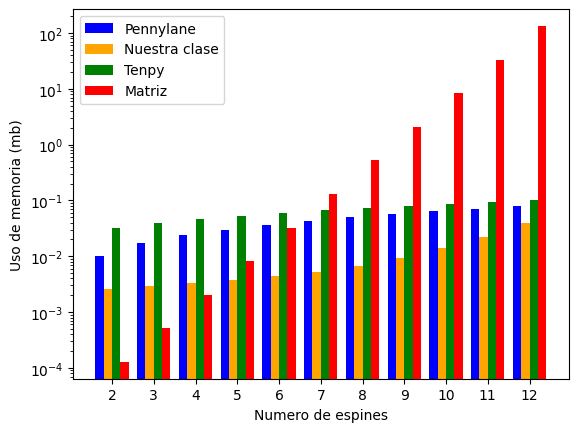
\includegraphics[width=0.7\textwidth]{figures/S4/spins/usomemoriahei.png}
\caption{\label{fig:23} Uso de memoria del hamiltoniano de espines XXX a diferente número de espines en (mb). Fuente: Elaboración propia}
\end{figure}

%%
%%
%%
\subsection{Análisis de tiempos}
El siguiente tema por tratar es el análisis de los tiempos de cómputo. Los cálculos que se muestran a continuación fueron realizados en un \textit{mac mini} con un \textit{chip Apple M2 Pro} con 32 GB de memoria Ram y 10 \textit{cores}, este dispositivo pertenece al grupo de simulaciones del departamento de física USM.

Dentro de este contexto, diagonalización exacta debe entenderse como el proceso de obtención de valores y vectores propios, para este caso utilizamos la rutina de la librería numpy \textit{numpy.linalg.eigh} que calcula estas cantidades de una matriz hermitiana. Para la DMRG, utilizamos la rutina \textit{tenpy.algorithms.dmrg.TwoSiteDMRGEngine} de la librería tenpy.


\subsubsection{Metodología}
Para cada hamiltoniano se elegirá valores de zonas de tipo 1, ya que en estas se tiene asegurada una convergencia ''rápida'' y una solución muy cercana al valor exacto. De esta forma podemos comparar el rendimiento de una forma justa. De trabajar en otras zonas, es claro que el tiempo está dado por el límite de iteraciones, lo cual no es lo que se busca. Es necesario mencionar que el tiempo considerado es desde el momento de ejecución del optimizador (para ejecutar el VQE) y las rutinas mencionadas anteriormente (de DMRG y diagonalización exacta) hasta finalizan, acá no se toma en cuenta el tiempo tomado en construir el hamiltoniano.

Los optimizadores serán informados dependiendo de cada caso, pero todos van a ser fijados con 100 iteraciones máximas y una tolerancia de $10^{-6}$, el resto de parámetros serán informados en cada hamiltoniano.

Finalmente, todos los cálculos son realizados utilizando CPU y con un solo proceso (no hay paralelización implementada, además del \textit{broadcasting} propio de numpy).

\subsubsection{Definición de los sistemas}

\underline{Hamiltoniano de moléculas}: 
Para el hamiltoniano molecular, se utilizará un arreglo 1D de hidrógenos, es decir, se van colocando hidrógenos en el eje Z, a una distancia de $1.3228$ (a.u) ($2.486864$ (angstrom)) entre cada uno, formando así la estructura 1D. Para este, se considera el \textit{basis set} ''sto-3g'', el \textit{ansatz} elegido es el UCCSD, ya que, basándonos en el análisis de la sección hamiltoniano-\textit{ansatz}, es el que mejor resultados da a medida que el sistema crece. Para el optimizador, se utilizará el gradiente genérico con \textit{learning rate} dé $0.3$.


\underline{Hamiltoniano de Fermi-Hubbard}: 
Del análisis de la sección hamiltoniano-\textit{ansatz} tenemos dos casos de interés, el primero es considerando $t=1$ y $U=0.0$ (\textit{tight binding}) y el segundo es $t=1$ y $U=0.2$ (Fermi-Hubbard), en ambos casos, se considerará en \textit{ansatz} k-UpCCGSD, y un optimizador genérico con \textit{learning rate} de $0.3$


\underline{Hamiltoniano de espín}: 
Del análisis de la sección hamiltoniano-\textit{ansatz} se elige un modelo XXX con una estructura de cadena, el valor del \textit{exchange} es dé $1.25$. El \textit{ansatz} que se utiliza es el \textit{hardware efficient} con una repetición. El optimizador elegido es un gradiente genérico con un \textit{learning rate} dé $0.3$.


\subsubsection{Resultados de tiempo de cómputo}

\underline{Hamiltoniano de moléculas}: 
\begin{figure}[H]
\centering
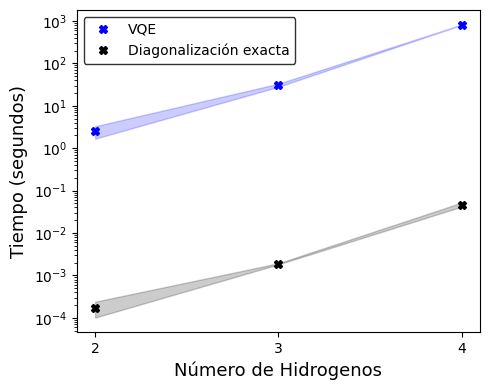
\includegraphics[width=0.7\textwidth]{figures/S4/moleculas/tiempomoleculas.png}
\caption{\label{fig:33} Tiempos de cómputo del estado de mínima energía en cadenas 1D de hidrógeno en segundos. Fuente: Elaboración propia}
\end{figure}

En la figura \ref{fig:33}, se puede observar el comportamiento de los tiempos de cómputo a medida que aumentamos el número de hidrógenos en la cadena. Si bien se tienen pocos puntos, se puede apreciar como ambos tiempos se comportan como líneas rectas paralelas (en escala logarítmica), en las cuales, el VQE tarda más que la diagonalización exacta.

Si entramos dentro de un análisis más detallado, encontramos que a medida que aumentamos el tamaño, el VQE requiere más ejecuciones ($5$, $16$, $67$ respectivamente), y el número de parámetros también aumenta ($3$, $8$, $26$ respectivamente).


\underline{Hamiltoniano de Fermi-Hubbard}: 
\begin{figure}[H]
\centering
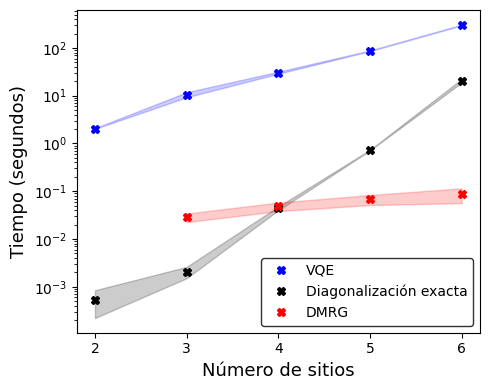
\includegraphics[width=0.7\textwidth]{figures/S4/tb/tiempotb.png}
\caption{\label{fig:34} Tiempos de cómputo del estado de mínima energía en el modelo de \textit{tight binding} en segundos. Fuente: Elaboración propia}
\end{figure}

En la figura \ref{fig:34} se puede ver el comportamiento de los tiempos de cómputo a medida que aumentamos el número de sitios en el modelo de \textit{tight binding}. El VQE se muestra como el que más tiempo tarda, con una tendencia lineal a medida que crece el sistema, por otro lado, la diagonalización exacta muestra tiempos menores, pero con una tendencia exponencial. Finalmente, DRMG muestra los mejores tiempos cuando crece el sistema con una tendencia logarítmica (recordando que el gráfico está en escala logarítmica). 

Para el VQE, se tiene que independiente del número de sitios, el circuito se tiene que ejecutar cuatro veces por llamada de la función de coste, y a medida que crece el sistema, el número de parámetros es $6$, $18$, $36$, $60$ y $90$ respectivamente.


\begin{figure}[H]
\centering
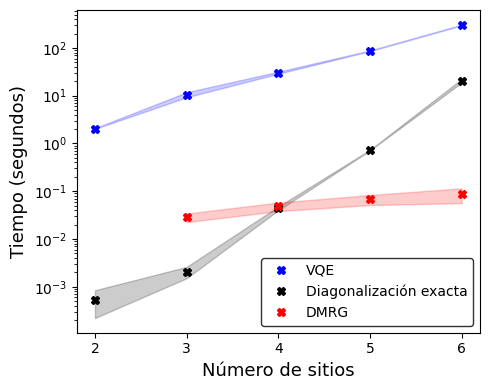
\includegraphics[width=0.7\textwidth]{figures/S4/fermi/tiempofb.png}
\caption{\label{fig:35} Tiempos de cómputo del estado de mínima energía en el modelo de Fermi-Hubbard en segundos. Fuente: Elaboración propia}
\end{figure}

Ahora, pasando al modelo de Fermi-Hubbard, ver figura \ref{fig:35}, tenemos comportamientos similares, ya que, en esencia ambos modelos son muy similares, solo se agregan nuevos términos. En temas de tiempo de ejecución, no existen diferencias sustanciales.

Si entramos a analizar el VQE, encontramos que el número de ejecuciones pasa a cinco y el número de parámetros se mantiene igual al de \textit{tight binding}.

\underline{Hamiltoniano de espín}: 

\begin{figure}[H]
\centering
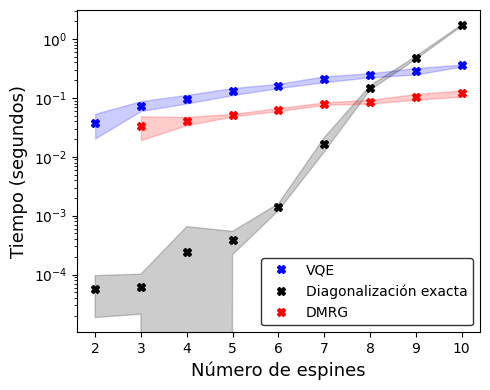
\includegraphics[width=0.7\textwidth]{figures/S4/spins/tiempoespines.png}
\caption{\label{fig:36} Tiempos de cómputo del estado de mínima energía en el modelo de Heisenberg en segundos. Fuente: Elaboración propia}
\end{figure}

Ahora, pasando al modelo de espines, ver figura \ref{fig:36}, tenemos nuevamente que el VQE es el que más tarda para sistemas de baja dimensionalidad, pero en sistemas de mediana dimensionalidad (sobre 8 espines), se ve que es mejor que la diagonalización exacta. El VQE muestra una tendencia entre lineal y logarítmica, mientras que diagonalización exacta tiene una tendencia que parece exponencial. Luego tenemos DMRG que tiene un comportamiento paralelo que el VQE, con la diferencia que ofrece tiempos menores.

Al igual que en el modelo anterior, el número de ejecuciones del circuito por cómputo de la función de coste es constante (tres ejecuciones), mientras que el número de parámetros si crece al aumentar el tamaño, este tiene un crecimiento lineal respecto al número de espines.







%%
%%
%%
%%
\subsection{Más allá del VQE}
En esta sección, el objetivo es realizar estudios más complejos utilizando el VQE, de manera más concreta, nos enfocaremos en dos tópicos, el primero es dinámica molecular en el sentido de relajación de estructuras y el segundo es simular los efectos de la temperatura en alguna estructura.

Respecto al primer tópico, la idea es colocar una molécula donde los elementos no están en sus respectivas distancias de equilibrio, y desde ese punto, utilizando el VQE, poder simular el movimiento molecular que permite que los átomos se muevan a sus distancias de equilibrio \cite{OptimizationStruture}.

Para el segundo tópico, la idea es poder realizar termodinámica usando ordenadores cuánticos utilizando algunos de los métodos definidos, para ello se busca calcular los todos los niveles de energía del sistema para poder calcular de forma clásica, semi clásica los efectos de la temperatura sobre algún observable como la magnetización o el calor especifico. 

Es importante destacar que acá no se busca analizar el uso de recursos (tiempo y memoria), acá solo nos interesa la calidad de ciertos valores de interés, los cuales serán indicados más adelante dependiendo del tópico.

\subsubsection{Metodología}
El objetivo de esta sección es proponer una metodología para poder llevar a cabo estudios de una forma metódica y estándar que permita comparar resultados de buena calidad.

Lo primero es el elegir los hiperparámetros adecuados (el \textit{ansatz} y el optimizador), entonces, dado un sistema, lo primero es elegir un conjunto de \textit{ansatzs} adecuados (que por el contexto tengan sentido utilizarlos), para comparar la capacidad del \textit{ansatz} utilizaremos el VQE con un optimizador genérico con configuraciones base y con un número distinto de repeticiones. La razón detrás de esto es que si el \textit{ansatz} no es capaz de capturar el estado de mínima energía, no va a ser capaz de capturar otras características. 

Una vez elegido el \textit{ansatz} lo siguiente es elegir el mejor optimizador basándonos en este \textit{ansatz}, como los pasos de optimización son costosos, el criterio de selección es a base de la tolerancia obtenida contra el número de pasos (en este caso, se prueban diferentes métodos y diferentes \textit{learning rates} si es que corresponde). Sobre la base de esto, es que podemos discriminar el mejor par de \textit{ansatz} y optimizador para el sistema y trabajar en las mejores condiciones.


Para la metodología del primer tópico, como se están trabajando con moléculas, la idea es elegir un estado cercano al mínimo ($\pm 0.3$ (ángstrom) de la distancia de equilibrio), ya que, por cómo se vio en la sección de ''Análisis de la relación hamiltoniano-\textit{ansatz}'' los \textit{ansatz} para moléculas tienen un buen funcionamiento cercano a la distancia de equilibrio. Para este tópico, se requieren dos optimizadores, uno para los parámetros del \textit{ansatz} y otro que va a representar el movimiento por el espacio (acercando o alejando los elementos). Como acá estamos dejando la molécula ''libre'', tenemos que repetir esta ejecución 10 veces para poder construir un promedio y una desviación estándar representativa, de esta forma se podrá comparar con el valor de distancia real, cabe mencionar, que acá no nos interesa tanto la calidad de la solución de la energía nos interesa la distancia molecular.

Ahora pensando a la metodología del segundo tópico, este se puede entender como un proceso de dos pasos, el primero es el poder capturar todos los niveles de energía y el segundo es el estimar la distribución de probabilidad de los estados. 

Para el primer caso, vamos a seguir el mismo procedimiento que el utilizado para las regiones de tipo 1, primero vamos a ver cuántas repeticiones del \textit{hardware efficient ansatz} se necesitan para capturar el estado de mínima energía, acá buscamos el número máximo de repeticiones que se puede seleccionar hasta que no se vea mejora (como el objetivo es capturar estados excitados, no podemos esperar que el \textit{ansatz} que captura el estado de mínima energía sea suficiente para capturar los excitados). Una vez seleccionado el número de repeticiones, podemos pasar a calcular los niveles excitados usando el VQD, acá vamos a repetir este cálculo 10 para tener un conjunto que represente la viabilidad a la hora de ejecutar el VQD. 

Para el segundo paso, vamos a utilizar cada una de las 10 repeticiones para construir la distribución de estados y calcular el calor especifico (generando así 10 distribuciones y 10 curvas de calor especifico). Esta distribución de estados se calcula de forma clásica calculando el producto $\exp{-E_i/k_b t}/\mathcal{Z}$ (siendo $E_i$ las energías obtenidas del VQD). La idea, es que estos resultados se comparen con los obtenidos de forma exacta (calculando los valores y vectores propios usando diagonalización exacta).

%El estudiante realizo una tesis en un area de frontera, de manera interdiciplinaria entre las ciencias computacionales y la física-química, en un campo recientemente abierto al mundo. Creo que debe publicarse.

\subsubsection{Definición de los sistemas}

\begin{figure}[H]
\centering
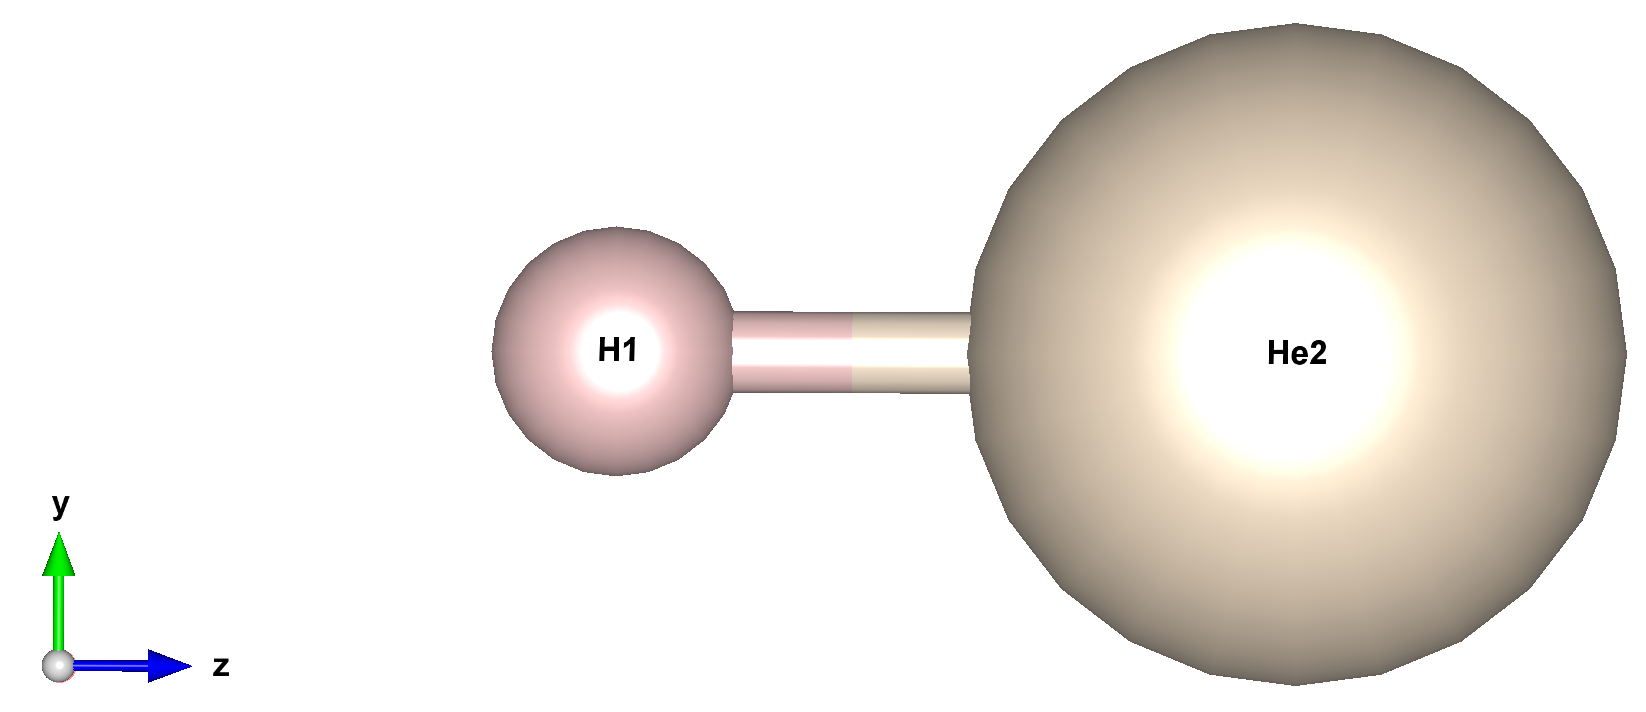
\includegraphics[width=0.5\textwidth]{figures/S4/moleculas/hhe.png}
\caption{\label{fig:hhe} Ion de helio hidrógeno con una distancia de enlace por el eje Z. Fuente: Elaboración propia}
\end{figure}


Para la optimización de las distancias, se tomará como sistema el ion de helio hidrógeno, ver figura \ref{fig:hhe}, este será construido usando el \textit{basis set} ''sto-3g'' a una distancia de $0.6$ (ángstrom) en el eje Z. Utilizando la CCCBDB \cite{CCCBDB}, sabemos que la distancia en equilibrio usando este \textit{basis set} es de $0.9295$ (ángstrom).

Para el análisis de temperatura, consideramos un modelo de espines XXX con 3 espines, con condiciones de borde abiertas y un \textit{exchange} $J = 1.0$ (eV).

\subsubsection{Resultados numéricos}

\underline{Optimización de estructuras}:
Comenzando con el ion de helio hidrógeno, este se puede considerar como un sistema de baja dimensionalidad (el espacio es más pequeño que el catión trihidrógeno), por lo tanto, considerando lo visto en la sección de '’Análisis de la relación hamiltoniano-\textit{ansatz}'', ambos \textit{ansatz} (UCCSD y k-UpCCGSD) van a tener un buen rendimiento. Dicho la elección del \textit{ansatz} pasa a ser algo más arbitrario, en este caso, se trabajará con el UCCSD (que fue el que mejor resultados dio para el catión trihidrógeno). Para el optimizador de los parámetros del \textit{ansatz} se usará el optimizador genérico con un \textit{learning rate} fijo dé $0.2$. 

\begin{figure}[H]
\centering
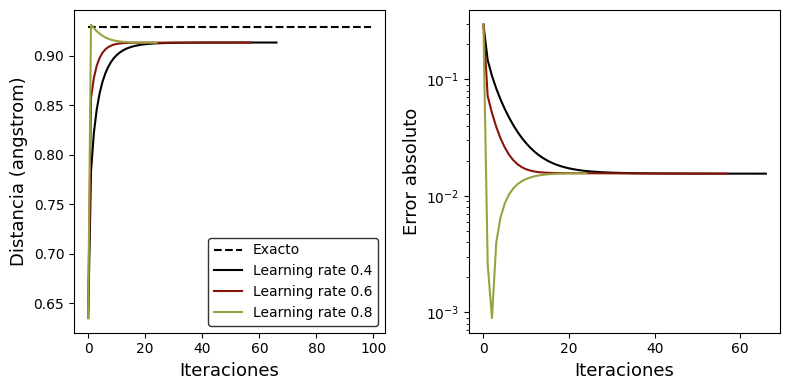
\includegraphics[width=0.8\textwidth]{figures/S4/moleculas/estructuras1.png}
\caption{\label{fig:41} VQE aplicado a cálculo de distancia molecular utilizando un optimizador genérico. Fuente: Elaboración propia}
\end{figure}

En la figura \ref{fig:42} se puede observar los resultados de con optimizador genérico con diferentes \textit{learning rates}. En ninguno de los casos, se observa que se alcance la distancia real, a pesar de la anomalía con el \textit{learning rate} $0.8$. Frente a esto, se cambia el optimizador por ADAM con un nuevo conjunto de \textit{learning rates} más pequeños (esto también implica que tengamos que aumentar el número de iteraciones máximas).

\begin{figure}[H]
\centering
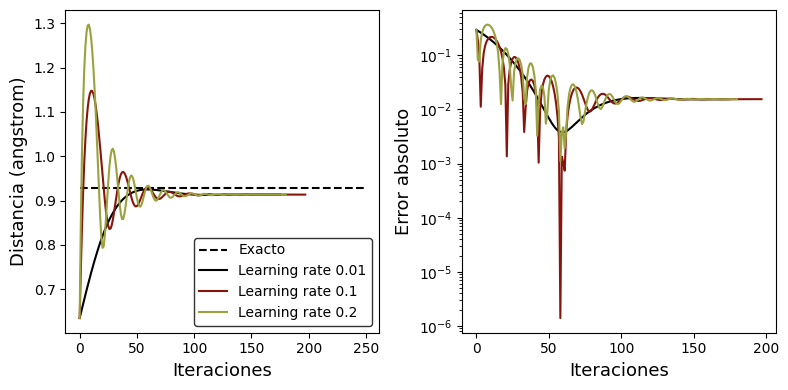
\includegraphics[width=0.8\textwidth]{figures/S4/moleculas/estructuras2.png}
\caption{\label{fig:42} VQE aplicado a cálculo de distancia molecular utilizando el optimizador ADAM. Fuente: Elaboración propia}
\end{figure}


Los efectos del optimizador se puede observar en la figura \ref{fig:42}, donde se pueden observar resultados similares a los obtenidos con el gradiente genérico, a pesar de la anomalía que se observa con el \textit{learning rate} $0.1$. Frente a esto, nos quedaremos con el gradiente genérico con \textit{learning rate} $0.6$ que nos entrega resultados similares en menor número de iteraciones.


\begin{figure}[H]
\centering
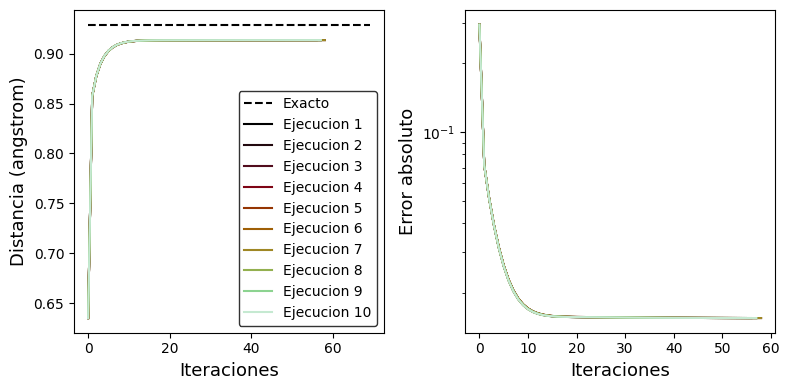
\includegraphics[width=0.8\textwidth]{figures/S4/moleculas/estructuradistancia.png}
\caption{\label{fig:43} VQE aplicado a cálculo de distancia molecular utilizando los mejores hiperparámetros. Fuente: Elaboración propia}
\end{figure}

\begin{figure}[H]
\centering
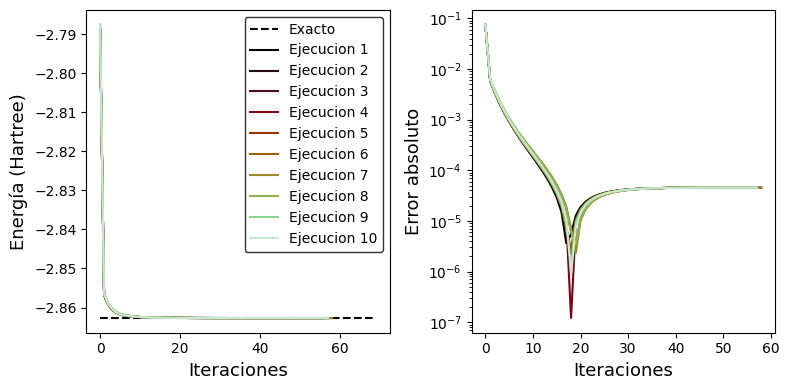
\includegraphics[width=0.8\textwidth]{figures/S4/moleculas/estructuraenergia.png}
\caption{\label{fig:44} VQE aplicado a cálculo de energía del estado de mínima energía utilizando los mejores hiperparámetros. Fuente: Elaboración propia}
\end{figure}


Dicho lo anterior, ahora que tenemos definidos los hiperparámetros, podemos analizar los resultados del sistema, las figuras \ref{fig:43} y \ref{fig:44} se puede observar la convergía de las diversas repeticiones en la energía y distancia del sistema respectivamente. En estas dos figuras se puede observar los efectos de la baja dimensionalidad (hay poca variabilidad entre ejecuciones), por otro lado, se observa una anomalía en el error absoluto de la energía obtenida (ver figura \ref{fig:44}) cerca de las 15 iteraciones, lo cual puede ser explicado como un efecto colateral de la convergencia de las distancias entre elementos. Por otro lado, si nos centramos en la figura \ref{fig:43}, es posible apreciar cómo no se alcanza la distancia de equilibrio, el error se estanca en un error absoluto de alrededor $10^{-1}$. 


\underline{Niveles excitados y temperatura}: 
Ahora respecto al sistema de espines, como acá estamos buscando capturar todos los niveles excitados, primero se tiene que hacer un análisis de las repeticiones del \textit{ansatz} para obtener la mayor cantidad posible de tal forma de poder asegurar que el \textit{ansatz} es capaz de capturar estados excitados. 

\begin{figure}[H]
\centering
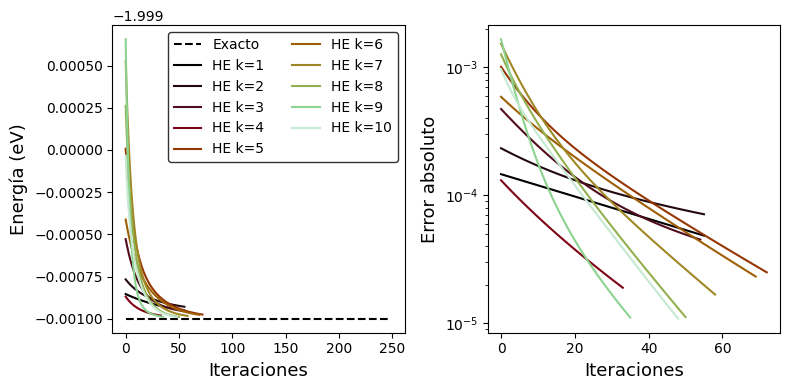
\includegraphics[width=0.8\textwidth]{figures/S4/spins/temperatura1.png}
\caption{\label{fig:45} VQE aplicado a modelo de espines considerando 3 espines con condiciones de borde abiertas. Fuente: Elaboración propia}
\end{figure}

En la figura \ref{fig:45} se puede observar el efecto de aumentar el número de repeticiones (para no tener efectos de oscilaciones en la convergencia, acá se redujo el \textit{learning rate} a $0.01$ y se aumentó el número de iteraciones a 250), en todos los casos se observa una convergencia, el error se reduce de manera casi lineal en escala logarítmica. Para este caso, nos quedaremos con 10 repeticiones para asegurar una buena captura de estados excitados.

\begin{figure}[H]
\centering
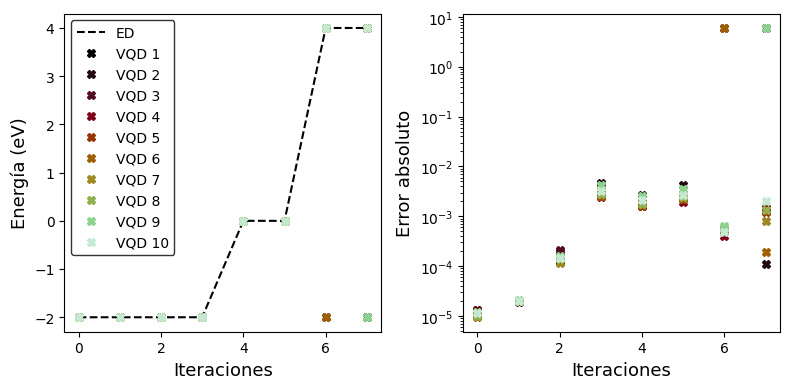
\includegraphics[width=0.8\textwidth]{figures/S4/spins/temperatura2.png}
\caption{\label{fig:46} VQD aplicado a modelo de Heisenberg de 3 espines con condiciones de borde abiertas. Fuente: Elaboración propia}
\end{figure}

Dicho lo anterior, nos quedaremos los hiperparámetros mencionados anteriormente para ejecutar el VQD. En la figura \ref{fig:46} se puede observar un resumen de los niveles obtenidos en las 10 ejecuciones del VQD. En varias ejecuciones se ve como se obtienen niveles erróneos que escapan del valor exacto (también se ve en la gráfica del error, donde en un par de casos llega a un error cercano a $10^{1}$), pero en general, se observa una buena captura de los estados excitados en las ejecuciones.

Visto que en gran parte de los casos el VQD funciona bien, podemos pasar a hablar de la estimación de la distribución de estados. Acá la idea es utilizar un enfoque híbrido para el cómputo de la distribución, donde se utilizan las energías obtenidas del VQD para calcular las exponenciales correspondientes. Acá consideraremos el conjunto de $[1, 2, 4, 8, 16, 32]$ (K) para calcular el calor especifico.

\begin{figure}[H]
\centering
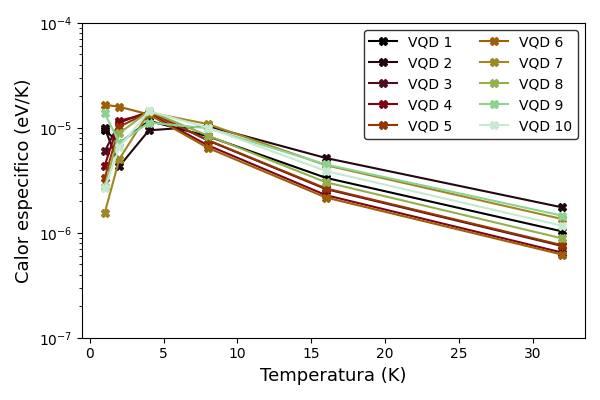
\includegraphics[width=0.8\textwidth]{figures/S4/spins/temperatura3.png}
\caption{\label{fig:47} Calor especificó calculado usando energías obtenidas del VQD. Fuente: Elaboración propia}
\end{figure}

En la figura \ref{fig:47} se puede observar el cálculo del calor específico para cada una de las ejecuciones del VQD, en la mayoría de los casos se observa un pequeño máximo para luego empezar a decaer. Esta cantidad no puede ser comparada con valores exactos por una indeterminación de las operaciones (algunos cálculos de exponenciales sufren de \textit{overflow} considerando \textit{float128}, haciendo que todos los valores sean retornados sean 0). Frente a esto, se tienen dos posibles conclusiones, respecto al fenómeno, se ve que se obtienen tendencias que son esperadas (cambios de fases) por efectos de las temperaturas, también podemos analizar respecto a su cercanía al valor 0, dentro de lo cual, estamos dentro de una tolerancia aceptable.

Independiente de esto, se puede observar como técnicas como el VQD nos pueden ser útil a la hora de tratar de estudiar observables termodinámicos.

